\ifdefined\manuscriptwithsupplement
\clearpage
\begingroup
\normalsize
\setcounter{section}{0}
\setcounter{table}{0}
\setcounter{figure}{0}
\setcounter{equation}{0}
\renewcommand{\thesection}{S\arabic{section}}
\renewcommand{\thetable}{S\arabic{table}}
\renewcommand{\thefigure}{S\arabic{figure}}
\renewcommand{\theequation}{S\arabic{equation}}
\renewcommand{\theHsection}{supp.\arabic{section}}
\renewcommand{\theHtable}{supp.\arabic{table}}
\renewcommand{\theHfigure}{supp.\arabic{figure}}
\renewcommand{\theHequation}{supp.\arabic{equation}}
\setlength{\emergencystretch}{2em}
\clubpenalty=10000
\widowpenalty=10000
\begin{center}
{\LARGE Supplementary Material:\\Benchmark Definitions, Execution Protocol, and Uncertainty\par}
\end{center}
\else
\documentclass{article}
\usepackage[T1]{fontenc}
\usepackage[utf8]{inputenc}
\usepackage[letterpaper,margin=1in]{geometry}
\usepackage{amsmath,amssymb,booktabs,placeins,xurl}
\usepackage{longtable,pdflscape,graphicx}
\renewcommand{\thefigure}{S\arabic{figure}}
\usepackage[authoryear,round,sort]{natbib}
\usepackage[hidelinks]{hyperref}
\renewcommand{\thetable}{S\arabic{table}}
\renewcommand{\theequation}{S\arabic{equation}}
\renewcommand{\thesection}{S\arabic{section}}
\setlength{\emergencystretch}{2em}
\clubpenalty=10000
\widowpenalty=10000
\title{Supplementary Material:\\Benchmark Definitions, Execution Protocol, and Uncertainty}
\author{}
\date{}
\setlength{\emergencystretch}{2em}
\begin{document}
\maketitle
\vspace{-2em}
\fi
The Grid-GDP functions are adapted from the Quantum Hamiltonian Descent collection; each instance is defined by its implemented expression and domain rather than its conventional name~\citep{qhdBenchmarks,rbfoptTestArchive}.

\section{Coordinate domains and normalization}\label{sec:supp-domains}
The coordinate mapping and objective normalization follow Section~\ifdefined\manuscriptwithsupplement\ref{sec:grid-gdp-formulation}\else3.1\fi{} of the main paper.
Both coordinate endpoints are included, and \(L\) and \(U\) are the minimum and maximum over the 961 lattice points.
All trigonometric arguments are in radians.
Full-precision normalization constants and target coordinates are archived in \nolinkurl{grid_inventory.json} (Section~\ref{sec:supp-data}).

\begin{table}[htbp]
\centering\small
\caption{Grid-GDP benchmark domains and target-set sizes.
Each problem uses a \(31\times31\) lattice with 961 configurations and 62 Boolean indicators.
\(n_{\rm target}\) counts lattice points with normalized objective \(F\leq10^{-5}\).}
\label{tab:grid-domains}
\begin{tabular}{llll}\toprule
Function & \(x\) domain & \(y\) domain & \(n_{\rm target}\)\\\midrule
Ackley & \([-5,5]\) & \([-5,5]\) & 1\\
Alpine 1 & \([0,10]\) & \([0,10]\) & 1\\
Alpine 2 & \([0,1000]\) & \([0,1000]\) & 1\\
Bohachevsky 2 & \([-100,100]\) & \([-100,100]\) & 1\\
Three-hump camel & \([-5,5]\) & \([-5,5]\) & 1\\
Csendes (squared variant) & \([-1,1]\) & \([-1,1]\) & 36\\
Deflected corrugated spring & \([0,10]\) & \([0,10]\) & 1\\
Drop-Wave & \([-5.12,5.12]\) & \([-5.12,5.12]\) & 1\\
Easom & \([-10,10]\) & \([-10,10]\) & 1\\
Griewank & \([-600,600]\) & \([-600,600]\) & 1\\
H\"older table & \([-10,10]\) & \([-10,10]\) & 4\\
Hosaki & \([0,5]\) & \([0,6]\) & 1\\
L\'evy & \([-10,10]\) & \([-10,10]\) & 2\\
L\'evy 13 & \([-10,10]\) & \([-10,10]\) & 4\\
Michalewicz & \([0,\pi]\) & \([0,\pi]\) & 1\\
Rastrigin & \([-5.12,5.12]\) & \([-5.12,5.12]\) & 1\\
Rosenbrock & \([-2,2]\) & \([-1,3]\) & 2\\
Shubert (historical variant) & \([0,10]\) & \([0,10]\) & 1\\
Styblinski--Tang & \([-5,5]\) & \([-5,5]\) & 1\\
Sum of squares & \([-10,10]\) & \([-10,10]\) & 1\\
Xin-She Yang 3 (historical variant) & \([-20,20]\) & \([-20,20]\) & 870\\\bottomrule
\end{tabular}
\end{table}

\FloatBarrier % \clearpage
\section{Grid-GDP objective functions}\label{sec:supp-objectives}
The implemented functions below use the domains in Table~\ref{tab:grid-domains}~\citep{rbfoptTestArchive}.

\subsection*{1. Ackley}
\begin{equation}\label{eq:supp-ackley}
\begin{aligned}
f(x,y)={}&-20\exp\!\left(-0.2\sqrt{\frac{x^2+y^2}{2}}\right)\\
&-\exp\!\left(\frac{\cos(2\pi x)+\cos(2\pi y)}{2}\right)+20+e.
\end{aligned}
\end{equation}

\subsection*{2. Alpine 1}
\begin{equation}\label{eq:supp-alpine1}
f(x,y)=|x\sin x+0.1x|+|y\sin y+0.1y|.
\end{equation}

\subsection*{3. Alpine 2}
\begin{equation}\label{eq:supp-alpine2}
f(x,y)=-\sqrt{xy}\,\sin x\sin y.
\end{equation}

\subsection*{4. Bohachevsky 2}
\begin{equation}\label{eq:supp-bohachevsky2}
f(x,y)=x^2+2y^2-0.3\cos(3\pi x)\cos(4\pi y)+0.3.
\end{equation}

\subsection*{5. Three-hump camel}
\begin{equation}\label{eq:supp-camel3}
f(x,y)=2x^2-1.05x^4+\frac{x^6}{6}+xy+y^2.
\end{equation}

\subsection*{6. Csendes (squared variant)}
\begin{equation}\label{eq:supp-csendes}
f(x,y)=c(x)+c(y),\qquad
c(t)=\begin{cases}
t^6\bigl[2+\sin(1/t)\bigr]^2,&t\ne0,\\
0,&t=0.
\end{cases}
\end{equation}
The GDP uses branch-fixed auxiliaries \(r_t=1/t\) for \(t\ne0\) and \(r_t=0\) otherwise, avoiding division by zero without an epsilon shift.

\subsection*{7. Deflected corrugated spring}
With \(r=\sqrt{(x-5)^2+(y-5)^2}\),
\begin{equation}\label{eq:supp-spring}
f(x,y)=0.1r^2-\cos(5r).
\end{equation}

\subsection*{8. Drop-Wave}
\begin{equation}\label{eq:supp-dropwave}
f(x,y)=-\frac{1+\cos\!\left(12\sqrt{x^2+y^2}\right)}{0.5(x^2+y^2)+2}.
\end{equation}

\subsection*{9. Easom}
\begin{equation}\label{eq:supp-easom}
f(x,y)=-\cos x\cos y\,\exp\!\left(-[(x-\pi)^2+(y-\pi)^2]\right).
\end{equation}

\subsection*{10. Griewank}
\begin{equation}\label{eq:supp-griewank}
f(x,y)=\frac{x^2+y^2}{4000}-\cos x\cos\!\left(\frac{y}{\sqrt{2}}\right)+1.
\end{equation}

\subsection*{11. H\"older table}
\begin{equation}\label{eq:supp-holder}
f(x,y)=-\left|\sin x\cos y\,
\exp\!\left(\left|1-\frac{\sqrt{x^2+y^2}}{\pi}\right|\right)\right|.
\end{equation}

\subsection*{12. Hosaki}
\begin{equation}\label{eq:supp-hosaki}
f(x,y)=\left(1-8x+7x^2-\frac{7}{3}x^3+\frac14x^4\right)y^2\exp(-y).
\end{equation}

\FloatBarrier % \clearpage
\subsection*{13. L\'evy}
Define \(w_x=1+(x-1)/4\) and \(w_y=1+(y-1)/4\).
Then
\begin{equation}\label{eq:supp-levy}
\begin{aligned}
f(x,y)={}&\sin^2(\pi w_x)\\
&+(w_x-1)^2\bigl[1+10\sin^2(\pi w_x+1)\bigr]\\
&+(w_y-1)^2\bigl[1+\sin^2(2\pi w_y)\bigr].
\end{aligned}
\end{equation}

\subsection*{14. L\'evy 13}
\begin{equation}\label{eq:supp-levy13}
\begin{aligned}
f(x,y)={}&\sin^2(3\pi x)+(x-1)^2\bigl[1+\sin^2(3\pi y)\bigr]\\
&+(y-1)^2\bigl[1+\sin^2(2\pi y)\bigr].
\end{aligned}
\end{equation}

\subsection*{15. Michalewicz}
\begin{equation}\label{eq:supp-michalewicz}
f(x,y)=-\sin x\,\sin^{20}\!\left(\frac{x^2}{\pi}\right)
-\sin y\,\sin^{20}\!\left(\frac{2y^2}{\pi}\right).
\end{equation}

\subsection*{16. Rastrigin}
\begin{equation}\label{eq:supp-rastrigin}
f(x,y)=x^2-10\cos(2\pi x)+y^2-10\cos(2\pi y)+20.
\end{equation}

\subsection*{17. Rosenbrock}
\begin{equation}\label{eq:supp-rosenbrock}
f(x,y)=(1-x)^2+100(y-x^2)^2.
\end{equation}

\subsection*{18. Shubert (historical variant)}
\begin{equation}\label{eq:supp-shubert}
\begin{aligned}
f(x,y)={}&\bigl[\cos(2x+1)+2\cos(3x+2)+3\cos(4x+3)\bigr]\\
&\times\bigl[\cos(2y+1)+\cos(y+2)\bigr].
\end{aligned}
\end{equation}

\FloatBarrier % \clearpage
\subsection*{19. Styblinski--Tang}
\begin{equation}\label{eq:supp-styblinski}
f(x,y)=\frac{1}{78}\,\frac12
\left(x^4-16x^2+5x+y^4-16y^2+5y\right).
\end{equation}

\subsection*{20. Sum of squares}
\begin{equation}\label{eq:supp-squares}
f(x,y)=x^2+2y^2.
\end{equation}

\subsection*{21. Xin-She Yang 3 (historical variant)}
\begin{equation}\label{eq:supp-xin}
f(x,y)=\exp\!\left(-\left[\left(\frac{x}{15}\right)^6+y^6\right]\right)
+2\exp\!\left(-(x^2+y^2)\right)\cos^2x\cos^2y.
\end{equation}

\FloatBarrier % \clearpage
\section{Executable protocol and implementation settings}\label{sec:supp-protocol}

Python and NumPy use the job seed, and \texttt{RBFOpt} also receives \nolinkurl{rand_seed}.
\texttt{BAM} exposes no separate native random-seed option: its process wrapper seeds Python/NumPy, while the Grid seed identifies the common initial design.
\texttt{FMQA-SA} uses three NumPy \nolinkurl{SeedSequence(seed)} streams for FM initialization, annealing, and uniform unseen-point fallback; each training or annealing invocation draws a seed from its stream.
\texttt{PyTorch} uses deterministic CPU operations and one thread.

Grid \texttt{D-SDA} enumerates \(L_\infty\) neighbors lexicographically from \((-1,0,1)\), excluding the zero direction and out-of-bounds points; ties select the first point.

The \texttt{RBFOpt} options are \nolinkurl{rbf=auto}, \nolinkurl{global_search_method=genetic}, \nolinkurl{do_init_strategy=False}, \nolinkurl{ga_base_population_size=400}, and \nolinkurl{ga_num_generations=20}.

\texttt{BAM} receives \nolinkurl{x0=None} and \nolinkurl{max_evals}=B-3; its local models use \texttt{ALAMO}/\texttt{BARON}, whose internal versions are not reported by the package.

The \texttt{FMQA-SA} time limit is checked between operations and through training/sampling callbacks.
Each FM uses identity activation, zero bias, and normal initial weights with mean zero and standard deviation \(0.01\).
Training uses Adam~\citep{kingma2015adam}, 1,000 full-batch epochs, mean squared error, and learning rate \(0.01\).
Coordinate \(\xi_j\) uses \(\lfloor\log_2 u_j\rfloor+1\) unsigned bits, where \(u_j>0\) is its upper bound; QUBO coefficients are divided by the largest absolute entry of the quadratic matrix.
D-Wave's \texttt{SimulatedAnnealingSampler} in \texttt{dwave-samplers} 1.6.0 uses 100 reads, 1,000 sweeps, and a geometric inverse-temperature schedule~\citep{dwaveSamplers}.
All process workers and the Grid \texttt{FMQA-SA} worker have a 2,100 s watchdog.
The Grid \texttt{RBFOpt}/\texttt{BAM} trace watchdogs are disabled (\nolinkurl{max_run_seconds=0}); archived Grid \texttt{D-SDA} uses budget, target, or local-search termination without an additional method-clock limit.

\subsection{Versions and independently timed process evaluations}\label{sec:supp-acceptance}
The recorded Python version is 3.11.16; other versions are given in the main paper\ifdefined\manuscriptwithsupplement\space(Section~\ref{sec:protocol})\fi.

The conventional GDP process models retain their archived initializations, including constructor defaults for \texttt{CSTR30}; the updated DFO evaluation table is identified separately in Section~\ref{sec:supp-data}.

The acceptance rule in \nolinkurl{gdp_models/evaluation.py} requires all of the following: a finite objective; termination in \{\texttt{optimal}, \texttt{locallyOptimal}, \texttt{globallyOptimal}\}; solver status other than \texttt{error} or \texttt{aborted}; interface status \texttt{SOLVESTAT}=1 and \texttt{MODELSTAT}\(\in\{1,2\}\); and a finite maximum primal violation no greater than \(10^{-5}\).
Time-limit, iteration-limit, evaluation-limit, and error outcomes are not accepted, even if a finite feasible candidate is available.

The primal check uses unscaled violations of original constraints and initialized-variable bounds, including constraint rows deactivated during preprocessing.
Nonfinite objectives, constraint bodies, or initialized-variable values preclude acceptance; unused uninitialized variables are skipped.
Preprocessing rejection or worker failure supplies no accepted objective.

The \texttt{CSTR} initializer \nolinkurl{cstr_box_ipopt.py:initialize_feasible} runs after preprocessing and checks the mass-balance/zero-recycle start at \(10^{-8}\) without changing constraints or bounds.
All process evaluations use cold starts; NLP solutions are not transferred between configurations.
Objectives, acceptance status, and NLP point costs are linked to the same recorded attempt by model, \texttt{CSTR} size, and coordinate, without successful-retry selection or cross-size time substitution.



\subsection{Observed proposal and initialization behavior}\label{sec:supp-proposals}
Table~\ref{tab:supp-fmqa-fallback} pools \texttt{FMQA-SA} proposals across budgets and seeds, excluding the shared initialization and including terminal callbacks.
Fallback supplies 52.89\% of process proposals; the uniform comparison evaluates the complete procedure, without isolating the contributions of learning, annealing, and fallback.

\begin{table}[htbp]
\centering\small
\caption{Recorded \texttt{FMQA-SA} uniform fallback by benchmark family.}
\label{tab:supp-fmqa-fallback}
\begin{tabular}{lrrrr}
\toprule
Family & Runs & Proposals & Fallbacks & Rate \\
\midrule
Grid & 1,050 & 51,450 & 9,522 & 18.51\% \\
\texttt{CSTR} & 60 & 1,350 & 369 & 27.33\% \\
\texttt{Column} & 10 & 100 & 86 & 86.00\% \\
\texttt{Dynamic} & 60 & 1,460 & 1,063 & 72.81\% \\
\texttt{Small Batch} & 10 & 70 & 58 & 82.86\% \\
Process total & 140 & 2,980 & 1,576 & 52.89\% \\
\bottomrule
\end{tabular}
\end{table}
\FloatBarrier

\section{Process model scale, units, and discrete decisions}\label{sec:supp-models}
Table~\ref{tab:supp-model-sizes} counts the original GDP before reformulation or presolve, including all active disjunct branches and fixed continuous variables.
\texttt{Dynamic} is discretized with 30 finite elements per stage and three Radau points.
Binary counts refer to the indicator variables already constructed by the model, before Boolean-to-binary conversion.
All nine models have zero additional nonbinary integer variables.

\begin{table}[htbp]
\centering
\small
\caption{Original process-model sizes.
\(n_c\): continuous variables; \(n_b\): binary variables; \(m_a\): algebraic constraints; \(m_l\): logical constraints; \(n_d\): disjunctions.}\label{tab:supp-model-sizes}
\begin{tabular}{lrrrrr}
\toprule
Model & \(n_c\) & \(n_b\) & \(m_a\) & \(m_l\) & \(n_d\)\\\midrule
\texttt{CSTR5} & 56 & 20 & 100 & 12 & 10 \\
\texttt{CSTR10} & 106 & 40 & 195 & 22 & 20 \\
\texttt{CSTR15} & 156 & 60 & 290 & 32 & 30 \\
\texttt{CSTR20} & 206 & 80 & 385 & 42 & 40 \\
\texttt{CSTR25} & 256 & 100 & 480 & 52 & 50 \\
\texttt{CSTR30} & 306 & 120 & 575 & 62 & 60 \\
\texttt{Column} & 446 & 30 & 637 & 16 & 15 \\
\texttt{Small Batch} & 19 & 18 & 34 & 3 & 9 \\
\texttt{Dynamic} & 1647 & 27 & 3276 & 31 & 9 \\
\bottomrule\end{tabular}\end{table}

\FloatBarrier

The \texttt{Column} objective is \(10^3(Q_c+Q_b)+10^3 n_{\rm active}\), the source model's weighted cost proxy rather than a newly estimated annualized cost.
The \texttt{Dynamic} objective is \(-\int_0^9 x(t)^2\,dt\).



\section{Process completion costs}\label{sec:supp-uncertainty}

Table~\ref{tab:process-tts99} reports completion costs for all 14 process conditions.
\begin{table}[p]
\centering
\caption{Median reconstructed full-run completion costs for all ten paired seeds per condition, including target misses, in seconds.}
\label{tab:process-tts99}
\small
\setlength{\tabcolsep}{6pt}
\par\smallskip\begin{tabular}{@{}lrccccc@{}}\toprule
Case & \(B\) & \texttt{D-SDA} & RBFOpt & BAM & \texttt{FMQA-SA} & Uniform \\\midrule
\texttt{Column} & 13 & 35.44 & 54.60 & 27.50 & 41.82 & 21.69 \\
\texttt{CSTR5} & 8 & 10.67 & 10.72 & 10.67 & 13.92 & 9.44 \\
\texttt{CSTR10} & 15 & 18.95 & 21.79 & 18.54 & 27.07 & 17.75 \\
\texttt{CSTR15} & 22 & 29.93 & 37.59 & 27.67 & 42.82 & 27.84 \\
\texttt{CSTR20} & 29 & 40.68 & 45.03 & 39.37 & 59.10 & 40.12 \\
\texttt{CSTR25} & 36 & 51.69 & 62.29 & 50.47 & 74.70 & 51.17 \\
\texttt{CSTR30} & 43 & 53.12 & 101.96 & 115.41 & 101.19 & 65.20 \\
\texttt{Small Batch} & 10 & 3.84 & 5.12 & 4.23 & 9.09 & 3.49 \\
\texttt{Dynamic} & 12 & 12.23 & 12.29 & 9.95 & 14.47 & 7.80 \\
\texttt{Dynamic} & 15 & 15.85 & 16.10 & 11.53 & 18.39 & 8.71 \\
\texttt{Dynamic} & 20 & 21.30 & 20.54 & 14.07 & 25.23 & 12.27 \\
\texttt{Dynamic} & 30 & 26.62 & 34.19 & 21.91 & 36.24 & 19.38 \\
\texttt{Dynamic} & 37 & 26.62 & 42.42 & 24.99 & 46.05 & 24.38 \\
\texttt{Dynamic} & 50 & 26.62 & 65.14 & 33.98 & 61.31 & 33.12 \\
\bottomrule\end{tabular}
\end{table}

Per-function Grid results at \(B=100\) and complete seed-level outcomes are available in the analysis files linked in Section~\ref{sec:supp-data}.

\FloatBarrier
\begingroup
\section{Data sources and reproducibility}\label{sec:supp-data}

The \href{https://github.com/SECQUOIA/Black-Box-for-GDP/tree/49d4bcbeb10fe49b74fe2333d27829046e93bf03}{publication snapshot} contains the source code, experimental data, analysis results, and reproduction instructions for the DFO and conventional GDP comparisons.
The updated \href{https://github.com/SECQUOIA/Black-Box-for-GDP/tree/329c6f93f4940436425582ae60323c0c9f95b581/results/gdpopt_scip_ipopt_analysis_20261030}{GDPopt analysis and execution records} contain the 63 Grid and 27 process runs configured with \texttt{SCIP} for MIP and \texttt{IPOPT} for NLP subproblems.
The three presolve-disabled LOA diagnostic runs are excluded.

\section{Feasibility and bound consistency of conventional GDP results}\label{sec:bound-audit}
Of the 45 conventional GDP runs in Table~\ref{tab:full-gdp}, 21 have flagged bounds (Table~\ref{tab:bound-audit}) relative to the checked solutions in Table~\ref{tab:witnesses}.
\david{we agreed that we are not calling algebraic the conventional methods for GDP}
\albert{Replaced algebraic with conventional GDP for the compared methods throughout the supplement, including the section heading.}
These results combine the 27 new \texttt{SCIP}--\texttt{IPOPT} GDPopt runs with the 18 retained direct \texttt{SCIP} runs.
Unrounded values, residuals, and source records are linked in Section~\ref{sec:supp-data}.

For each minimization model, let \(f_w\) be the recorded objective of its best independently checked saved feasible solution, and let \(L\) denote a reported lower bound.
We apply the same rule to all five methods:
\begin{equation}
 \tau_w=10^{-5}\max\{1,|f_w|\},\qquad
 \Delta=L-f_w,\qquad \rho=\Delta/\tau_w,\qquad
 \dagger\ \Longleftrightarrow\ \rho>1.
\end{equation}
Missing lower bounds remain missing, not zero.

Saved vectors are loaded into the original GDP to reevaluate objectives and check active constraints, variable bounds, integrality, disjunctions, and logical validity without optimization.
Violations are unscaled original-equation residuals, not reformulation residuals.
All 43 saved feasible vectors satisfy the \(10^{-5}\) threshold; the largest violation is \(9.90\times10^{-7}\).
The two Big-\(M\) runs without accepted feasible solutions remain in the 45-run denominator.
This numerical check establishes neither exact feasibility nor global optimality.

Eight of the 21 discrepancies are only 1.09--3.54 times the tolerance and are sensitive to numerical feasibility conventions.
These conflicting bounds and \nolinkurl{optimal} reports provide no independent global certificate or intrinsic method ranking; their cause in GDPopt or its subsolvers remains unresolved.

\par\endgroup
\begin{table}[htbp]
\centering
\caption{Reported lower bounds exceeding checked feasible objectives (\(\rho>1\)).}\label{tab:bound-audit}
\setlength{\tabcolsep}{4pt}
\begin{tabular}{lllrrlr}
\toprule
ID & Model & Method & Reported \(L\) & \(v_{\max}\) & C & \(\rho\)\\\midrule
S01 & \texttt{CSTR5} & RIC & 3.06201 & 2.60e-11 & C01 & 1.29\(^{\dagger}\) \\
S02 & \texttt{CSTR5} & GLOA & 3.13020 & 9.85e-12 & C01 & 2.23e+3\(^{\dagger}\) \\
S03 & \texttt{CSTR5} & LOA & 3.06201 & 2.60e-11 & C01 & 1.29\(^{\dagger}\) \\
S05 & \texttt{CSTR5} & Hull & 3.06201 & 9.34e-7 & C01 & 1.09\(^{\dagger}\) \\
S06 & \texttt{CSTR10} & RIC & 2.96605 & 1.62e-10 & C02 & 2.65e+3\(^{\dagger}\) \\
S07 & \texttt{CSTR10} & GLOA & 3.44796 & 3.11e-15 & C02 & 1.93e+4\(^{\dagger}\) \\
S08 & \texttt{CSTR10} & LOA & 2.96605 & 1.62e-10 & C02 & 2.65e+3\(^{\dagger}\) \\
S10 & \texttt{CSTR10} & Hull & 2.88951 & 9.37e-7 & C02 & 3.54\(^{\dagger}\) \\
S11 & \texttt{CSTR15} & RIC & 2.82939 & 1.33e-15 & C03 & 1.30\(^{\dagger}\) \\
S12 & \texttt{CSTR15} & GLOA & 3.56196 & 1.01e-15 & C03 & 2.59e+4\(^{\dagger}\) \\
S13 & \texttt{CSTR15} & LOA & 2.82939 & 1.33e-15 & C03 & 1.30\(^{\dagger}\) \\
S16 & \texttt{CSTR20} & RIC & 2.79941 & 1.58e-15 & C04 & 1.67\(^{\dagger}\) \\
S17 & \texttt{CSTR20} & GLOA & 3.61612 & 4.60e-11 & C04 & 2.92e+4\(^{\dagger}\) \\
S18 & \texttt{CSTR20} & LOA & 2.79941 & 1.58e-15 & C04 & 1.67\(^{\dagger}\) \\
S21 & \texttt{CSTR25} & RIC & 2.79125 & 1.38e-10 & C05 & 3.53e+2\(^{\dagger}\) \\
S22 & \texttt{CSTR25} & GLOA & 3.64786 & 2.22e-14 & C05 & 3.12e+4\(^{\dagger}\) \\
S27 & \texttt{CSTR30} & GLOA & 3.66872 & 7.11e-15 & C06 & 3.25e+4\(^{\dagger}\) \\
S32 & \texttt{Column} & GLOA & 20355.1 & 1.15e-13 & C07 & 4.65e+3\(^{\dagger}\) \\
S35 & \texttt{Column} & Hull & 20044.2 & 1.00e-8 & C07 & 3.06e+3\(^{\dagger}\) \\
S42 & \texttt{Dynamic} & GLOA & -197.140 & 9.85e-12 & C09 & 7.01e+3\(^{\dagger}\) \\
S45 & \texttt{Dynamic} & Hull & -196.931 & 1.00e-7 & C09 & 7.11e+3\(^{\dagger}\) \\
\bottomrule
\end{tabular}
\par\smallskip
\begin{minipage}{0.95\textwidth}\footnotesize
C identifies the comparison solution in Table~\ref{tab:witnesses}.
Displayed values are rounded; flags use unrounded values.
\end{minipage}
\end{table}
\david{something is wrong here, it appears as if there were two table captions}
\albert{Shortened the caption and moved the explanation below the table, with this review comment outside the caption.}
\FloatBarrier % \clearpage
\begingroup
\begin{table}[htbp]\centering\small
\caption{Checked saved comparison solutions; displayed values are rounded.}\label{tab:witnesses}
\setlength{\tabcolsep}{4pt}
\begin{tabular}{lllrr}\toprule
ID & Model & Method & Recorded \(f_w\) & \(v_{\max}\)\\\midrule
C01 & \texttt{CSTR5} & Big-\(M\) & 3.06198 & 9.40e-7 \\
C02 & \texttt{CSTR10} & Big-\(M\) & 2.88941 & 9.76e-7 \\
C03 & \texttt{CSTR15} & Hull & 2.82936 & 9.47e-7 \\
C04 & \texttt{CSTR20} & Hull & 2.79936 & 9.90e-7 \\
C05 & \texttt{CSTR25} & Hull & 2.78143 & 9.90e-7 \\
C06 & \texttt{CSTR30} & Big-\(M\) & 2.76957 & 9.68e-9 \\
C07 & \texttt{Column} & RIC & 19449.9 & 1.01e-13 \\
C08 & \texttt{Small Batch} & Big-\(M\) & 167428 & 9.00e-7 \\
C09 & \texttt{Dynamic} & Big-\(M\) & -212.009 & 1.00e-7 \\
\bottomrule\end{tabular}\end{table}

\paragraph{Additional tightened-feasibility check for \texttt{CSTR15}.}
An \texttt{IPOPT} 3.14.19 solve retained the archived LOA witness W03's discrete configuration and starting values and targeted an original-GDP residual of \(10^{-8}\)~\citep{rbfoptTestArchive}.
W03 is distinct from the current \texttt{SCIP} comparison solution C03.
Only exactly satisfied constant rows were omitted from the computational clone; the independent check retained all original constraints.
The returned objective was \(2.82939\), with maximum unscaled violation \(1.11\times10^{-16}\).
The new GLOA lower bound exceeds this objective by \(0.732565\), or approximately \(2.59\times10^4\) times the audit tolerance.
The discrepancy persists under the tighter check, but its cause remains unresolved.

\paragraph{Additional formulation check for \texttt{Dynamic} Hull.}
The saved Big-\(M\) point has objective \(-212.009\), approximately \(15.0776\) below the Hull lower bound \(-196.931\).
It satisfies both the original GDP and a reconstructed Hull formulation at \(10^{-5}\), with maximum violation approximately \(10^{-7}\).
The cause of the discrepancy remains unresolved.
\david{This is more of an implementation detail, why including it?}
\albert{Removed the export and implementation details, retaining only the feasibility check relevant to the reported bound.}

\FloatBarrier
\par\endgroup

\FloatBarrier % \clearpage
\section{Additional candidate-search and sampling comparisons}\label{sec:supp-additional}

\subsection{Paired differences and sampling controls}
The paired comparisons quantify differences in target-hit rates under shared initial designs, matching case, budget, and seed.
Positive differences favor the first method and are expressed in percentage points.
For Grid, the descriptive percentile bootstrap resamples the 21 intact function vectors, each containing ten paired seed differences, rather than treating 210 observations as exchangeable Bernoulli draws.
For Process, paired seeds are resampled within each of the 14 conditions; the six related \texttt{Dynamic} budgets are not pooled for inference.
The seed is 20261020 with 2,000 bootstrap replications and deterministic case/seed ordering.
Intervals are exploratory and unadjusted for multiple comparisons; ten-seed boundary cases may yield degenerate intervals, and zero inclusion does not establish equivalence.

An interval entirely above zero favors the first method under this resampling; an interval spanning zero leaves the direction uncertain.
There is no preset cutoff for practical importance.
For example, \texttt{BAM} matches its prefix control at \(B=10\) but exceeds it by 10.95 percentage points at \(B=100\), so initial sampling alone does not account for its final target-hit rate.
\david{SO what does this mean? WHy are you reporting this? If the difference is greater than a value does it mean something?}
\albert{Explained the sign and interval interpretation and used the BAM-prefix comparison to show why the paired results are reported.}

\begin{table}[htbp]\centering\small
\caption{Selected paired success differences, in percentage points.
The first method minus the second defines the sign; Process intervals concern the stated condition only.}
\textbf{Grid}\par\smallskip
\begin{tabular}{rlrr}\toprule
\(B\) & Contrast & Difference & 95\% interval\\\midrule
10 & \texttt{RBFOpt} -- Uniform & 13.33 & [5.71, 24.29] \\
100 & \texttt{RBFOpt} -- Uniform & 60.00 & [42.86, 75.71] \\
10 & \texttt{BAM} -- \texttt{BAM}-prefix control & 0.00 & [0.00, 0.00] \\
100 & \texttt{BAM} -- \texttt{BAM}-prefix control & 10.95 & [0.48, 23.81] \\
10 & \texttt{FMQA-SA} -- Uniform & 0.95 & [-0.95, 2.86] \\
100 & \texttt{FMQA-SA} -- Uniform & 40.00 & [28.57, 52.38] \\
10 & \texttt{D-SDA} -- \texttt{RBFOpt} & -13.81 & [-24.29, -6.19] \\
100 & \texttt{D-SDA} -- \texttt{RBFOpt} & -33.33 & [-48.10, -19.52] \\
\bottomrule\end{tabular}
\par\medskip
\textbf{Process: ten paired seeds per condition}\par\smallskip
\begin{tabular}{lrcrrr}\toprule
Case & \(B\) & Contrast & Outcomes & Difference & 95\% interval\\\midrule
\texttt{Dynamic} & 12 & \texttt{RBFOpt} -- \texttt{D-SDA} & 4/6/0/0 & 60 & [30, 90] \\
\texttt{Small Batch} & 10 & \texttt{FMQA-SA} -- Uniform & 2/4/2/2 & 20 & [-30, 60] \\
\bottomrule\end{tabular}
\par\smallskip
\begin{minipage}{0.95\textwidth}\footnotesize
Outcomes list both successful / first only / second only / neither successful.
\end{minipage}
\end{table}
\FloatBarrier

\subsection{Grid suite exclusions}
Excluding Xin-She Yang~3 and Bohachevsky~2 preserves the main descriptive pattern.
For the sampled Bohachevsky~2 lattice, \(\cos(3\pi a_i)=1\) at every coordinate, leaving an objective nearly redundant with sampled Sum of Squares after normalization.
Without both functions, \(B=100\) rates are 79.5\% for \texttt{RBFOpt}, 66.8\% for \texttt{BAM}, 57.9\% for \texttt{FMQA-SA}, 54.7\% for the \texttt{BAM}-prefix control, 42.6\% for \texttt{D-SDA}, and 17.9\% for uniform.
At \(B=10\), \texttt{BAM} and its prefix control each retain 47.9\%, compared with \texttt{RBFOpt} 15.8\%.


\david{This section is irrelevant, if the QUBOs were not saved, then just repeat the whole experiment and have it cleanly worked out}
\albert{Removed the reconstructed FMQA diagnostics and their main-text reference; no experiment was rerun and no validation of unsaved historical weights or QUBOs is claimed.}


\clearpage
\section{Joint comparison with conventional GDP methods}
\label{sec:supp-joint-comparison}
Figure~\ref{fig:joint-remaining-completion} compares the eight process conditions not shown in the main joint completion-time figure.
Each DFO condition has ten seeds, whereas each conventional GDP method has one run per problem.
Timing and target criteria follow Figure~\ifdefined\manuscriptwithsupplement\ref{fig:process-completion}\else3\fi{} of the main paper.
Table~\ref{tab:full-gdp} reports all nine models, including final objectives and termination flags.

\begin{table}[htbp]
\centering
\caption{Full-process-GDP results from one run per method and model.
Entries report the final objective and measured full-run completion time (s) in parentheses, including model-template preparation.
\texttt{GDPOpt} uses \texttt{SCIP} for master problems and \texttt{IPOPT} for NLP subproblems; Big-\(M\) and Hull retain their \texttt{SCIP} results.
Bold marks the lowest objective in each row and ties within \(10^{-5}\max\{1,|f_{\min}|\}\), where \(f_{\min}\) is the lowest objective in that row.
Feasibility means numerical feasibility under the original-GDP residual test at \(10^{-5}\), not exact feasibility.}
\label{tab:full-gdp}
\normalsize
\setlength{\tabcolsep}{5pt}
\renewcommand{\arraystretch}{1.08}
\begin{tabular}{@{}lccccc@{}}
\toprule
Model & RIC & GLOA & LOA & Big-\(M\) & Hull \\
\midrule
\texttt{CSTR5} & \makecell{3.06201\({}^{\dagger}\)\\(15.38)} & \makecell{3.13020\({}^{\dagger\ddagger}\)\\(4.57)} & \makecell{3.06201\({}^{\dagger}\)\\(24.58)} & \makecell{\textbf{3.06198}\\(53.68)} & \makecell{3.06201\({}^{\dagger}\)\\(15.43)} \\
\texttt{CSTR10} & \makecell{2.96605\({}^{\dagger\ddagger}\)\\(134.31)} & \makecell{3.44796\({}^{\dagger\ddagger}\)\\(3.10)} & \makecell{2.96605\({}^{\dagger\ddagger}\)\\(140.38)} & \makecell{\textbf{2.88941}\\(771.36)} & \makecell{2.88951\({}^{\dagger}\)\\(71.63)} \\
\texttt{CSTR15} & \makecell{2.82939\({}^{\dagger}\)\\(283.77)} & \makecell{3.56196\({}^{\dagger\ddagger}\)\\(6.17)} & \makecell{2.82939\({}^{\dagger}\)\\(445.43)} & \makecell{-\({}^{\mathrm{TL}}\)\\(1790.95)} & \makecell{\textbf{2.82936}\\(284.63)} \\
\texttt{CSTR20} & \makecell{2.79941\({}^{\dagger}\)\\(607.72)} & \makecell{3.61612\({}^{\dagger\ddagger}\)\\(7.46)} & \makecell{2.79941\({}^{\dagger}\)\\(733.53)} & \makecell{2.80413\({}^{\mathrm{TL}}\)\\(1792.44)} & \makecell{\textbf{2.79936}\\(1150.67)} \\
\texttt{CSTR25} & \makecell{2.79125\({}^{\dagger\ddagger}\)\\(1042.79)} & \makecell{3.64786\({}^{\dagger\ddagger}\)\\(5.20)} & \makecell{2.79125\({}^{\mathrm{TL}}\)\\(1790.35)} & \makecell{2.78771\({}^{\mathrm{TL}}\)\\(1792.33)} & \makecell{\textbf{2.78143}\\(1701.75)} \\
\texttt{CSTR30} & \makecell{2.77162\({}^{\mathrm{TL}}\)\\(1793.35)} & \makecell{3.66872\({}^{\dagger\ddagger}\)\\(5.52)} & \makecell{2.87314\({}^{\mathrm{TL}}\)\\(1798.05)} & \makecell{\textbf{2.76957}\({}^{\mathrm{TL}}\)\\(1791.82)} & \makecell{\textbf{2.76957}\({}^{\mathrm{TL}}\)\\(1792.56)} \\
\texttt{Column} & \makecell{\textbf{19449.9}\\(124.03)} & \makecell{20355.1\({}^{\dagger\ddagger}\)\\(42.41)} & \makecell{\textbf{19449.9}\\(199.22)} & \makecell{-\({}^{\mathrm{TL}}\)\\(1792.83)} & \makecell{22271.5\({}^{\mathrm{TL}\dagger}\)\\(1792.76)} \\
\texttt{Dynamic} & \makecell{\textbf{-212.009}\\(149.39)} & \makecell{-197.140\({}^{\dagger\ddagger}\)\\(238.96)} & \makecell{\textbf{-212.009}\\(550.49)} & \makecell{\textbf{-212.009}\({}^{\mathrm{TL}}\)\\(1791.75)} & \makecell{-196.931\({}^{\dagger\ddagger}\)\\(921.28)} \\
\texttt{Small Batch} & \makecell{\textbf{167428}\\(13.15)} & \makecell{\textbf{167428}\\(10.32)} & \makecell{\textbf{167428}\\(5.61)} & \makecell{\textbf{167428}\\(0.51)} & \makecell{\textbf{167428}\\(0.50)} \\
\bottomrule
\end{tabular}
\par\vspace{3pt}
\begin{minipage}{0.99\linewidth}
\small
TL: reported \texttt{maxTimeLimit} under the configured 1,800~s limit; measured times are retained, including values below 1,800~s.
Runs without TL report \texttt{optimal}.
\par
Dash: no accepted feasible solution.
\par
\(\dagger\): reported lower bound exceeds the best checked saved numerically feasible objective \(f\) by more than \(10^{-5}\max\{1,|f|\}\).
\par
\(\ddagger\): reference target missed despite reported \texttt{optimal} and a better checked numerically feasible solution.
\david{SOmetimes you call it target, sometimes lookup reference, unify this}
\albert{Used reference target for the success criterion; lookup now refers only to access to stored configuration responses.}
\end{minipage}
\end{table}
\FloatBarrier

\begin{table}[htbp]\centering\small
\caption{NLP workload in the process comparisons with \texttt{SCIP}--\texttt{IPOPT} GDPopt.
DFO entries are median counts of corresponding fixed-configuration NLP evaluations over ten seeds; GDPopt entries count confirmed IPOPT NLP interface calls in one run.
Logical and preprocessing rejections are excluded; rejected NLP returns are retained.
These counts are not internal solver iterations or equally costly subproblems.}
\label{tab:joint-nlp-workload}
\setlength{\tabcolsep}{3.5pt}
\begin{tabular}{lrrrrrrrrr}\toprule
Case & \(B\) & D-SDA & RBFOpt & BAM & FMQA-SA & Uniform & GLOA & LOA & RIC\\\midrule
CSTR5 & 8 & 6 & 6 & 6 & 5.5 & 4.5 & 4 & 15 & 15 \\
CSTR10 & 15 & 10 & 12 & 8.5 & 9 & 7.5 & 2 & 55 & 55 \\
CSTR15 & 22 & 17 & 16.5 & 11 & 15 & 11 & 4 & 120 & 120 \\
CSTR20 & 29 & 21 & 20.5 & 17 & 17.5 & 15.5 & 4 & 210 & 210 \\
CSTR25 & 36 & 25 & 25.5 & 18.5 & 23 & 21 & 2 & 315 & 325 \\
CSTR30 & 43 & 26.5 & 31.5 & 21.5 & 30.5 & 21.5 & 2 & 243 & 455 \\
Column & 13 & 11 & 12 & 7.5 & 7 & 7 & 18 & 38 & 38 \\
Small Batch & 10 & 4.5 & 6 & 5 & 5 & 4 & 12 & 5 & 12 \\
Dynamic & 12 & 10 & 10 & 8 & 6.5 & 6 & 20 & 37 & 37 \\
Dynamic & 15 & 13 & 13 & 9 & 8 & 6.5 & 20 & 37 & 37 \\
Dynamic & 20 & 17.5 & 16 & 11 & 11 & 9.5 & 20 & 37 & 37 \\
Dynamic & 30 & 22 & 21 & 17 & 14.5 & 15 & 20 & 37 & 37 \\
Dynamic & 37 & 22 & 25 & 19 & 19 & 19 & 20 & 37 & 37 \\
Dynamic & 50 & 22 & 31 & 26 & 24.5 & 26 & 20 & 37 & 37 \\
\bottomrule\end{tabular}
\par\smallskip
\begin{minipage}{0.98\linewidth}\footnotesize
The same single Dynamic GDPopt execution is repeated across budget rows for reference.
Internal NLP counts for direct Big-\(M\) and Hull are unavailable and are not treated as zero.
\end{minipage}
\end{table}
\FloatBarrier

\begin{figure}[p]
\centering
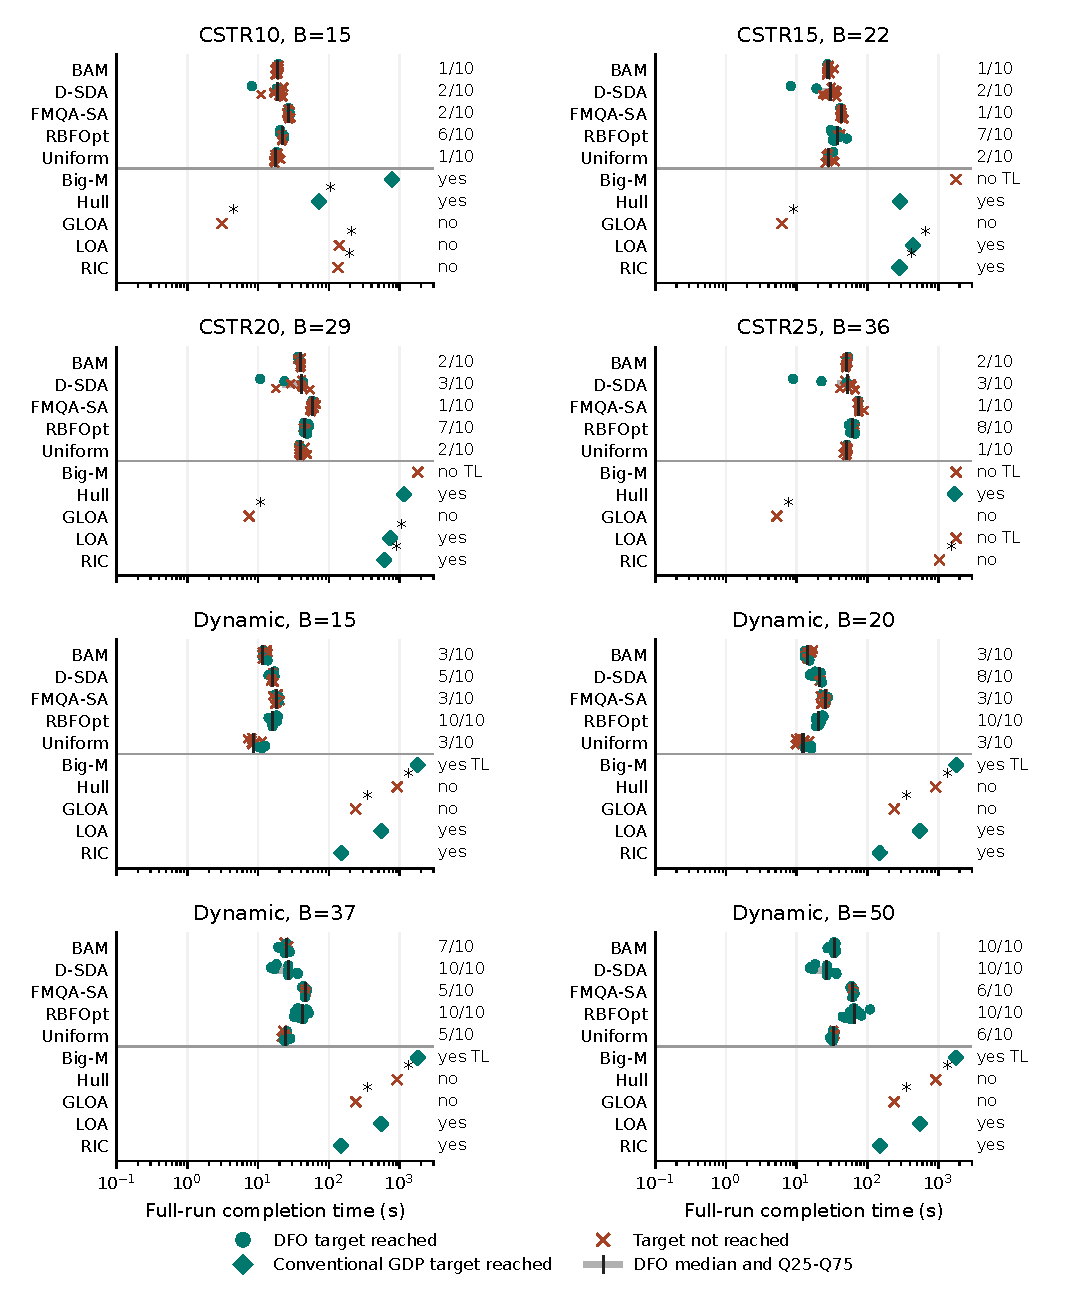
\includegraphics[width=\linewidth]{figures/joint_remaining_completion.pdf}
\caption{Joint full-run completion-time comparison for the eight additional process conditions.
Dots show successful DFO seeds, diamonds successful single conventional runs, and crosses target misses.
Gray segments and ticks show Q25--Q75 and medians across all ten DFO seeds.
TL denotes time-limit termination; asterisks mark bound inconsistencies (Section~\ref{sec:bound-audit}).
The Dynamic panels reuse the same conventional observations.
}
\label{fig:joint-remaining-completion}
\end{figure}
\FloatBarrier


\ifdefined\manuscriptwithsupplement
\FloatBarrier % \clearpage
\endgroup
\let\finishsupplement\relax
\else
\bibliographystyle{elsarticle-harv}
\bibliography{reference}
\def\finishsupplement{\end{document}}
\fi
\finishsupplement
